\documentclass[10pt,letterpaper]{article}

\usepackage[margin=0.82in,headheight=14pt]{geometry}
\usepackage{lmodern}
\renewcommand{\familydefault}{\sfdefault}
\usepackage{microtype}
\usepackage{amsmath}
\usepackage{graphicx}
\usepackage{booktabs}
\usepackage{tabularx}
\usepackage{array}
\usepackage{float}
\usepackage{enumitem}
\usepackage[table]{xcolor}
\usepackage{titlesec}
\usepackage{fancyhdr}
\usepackage{hyperref}

\definecolor{navy}{HTML}{17365D}
\definecolor{blue}{HTML}{2E75B6}
\definecolor{lightblue}{HTML}{EAF2F8}
\definecolor{graytext}{HTML}{4A5568}
\hypersetup{colorlinks=true,linkcolor=navy,urlcolor=blue}
\setlength{\parindent}{0pt}
\setlength{\parskip}{5pt}
\setlist{nosep,leftmargin=1.35em}
\titleformat{\section}{\Large\bfseries\color{navy}}{}{0pt}{}
\titleformat{\subsection}{\large\bfseries\color{blue}}{}{0pt}{}
\titlespacing*{\section}{0pt}{10pt}{5pt}
\titlespacing*{\subsection}{0pt}{8pt}{3pt}
\pagestyle{fancy}
\fancyhf{}
\fancyhead[L]{\small\color{graytext}CS683 Programming Assignment 1}
\fancyhead[R]{\small\color{graytext}Task 1: 2D Convolution}
\fancyfoot[C]{\small\thepage}
\renewcommand{\headrulewidth}{0.3pt}

\newcommand{\fig}[2]{%
  \begin{figure}[H]
    \centering
    \includegraphics[width=0.83\textwidth]{#1}
    \caption{#2}
  \end{figure}
}

\begin{document}

\hypersetup{pageanchor=false}
\begin{titlepage}
\thispagestyle{empty}
\vspace*{1.0in}
{\color{blue}\rule{\textwidth}{2.5pt}}\\[0.35in]
{\fontsize{30}{36}\selectfont\bfseries\color{navy} Task 1: Hardware-Conscious\\[3pt]2D Convolution}\par
\vspace{0.28in}
{\Large CS683 Programming Assignment 1}\par
\vspace{0.10in}
{\large Dhurandhar Programming}\par
\vfill
{\large Advanced Computer Architecture}\par
{\large Autumn 2026}\par
\vspace{0.18in}
{\large 5 September 2026}\par
\vspace{0.55in}
{\color{blue}\rule{\textwidth}{1pt}}
\end{titlepage}
\hypersetup{pageanchor=true}
\setcounter{page}{1}

\section{Executive summary}

This report evaluates loop reordering, manual loop unrolling, cache tiling, and explicit SIMD for single-channel, zero-padded 2D convolution. All submitted kernels match the supplied naive reference within the required absolute tolerance of $10^{-3}$. On the graded $2048\times2048$, $K=3$ workload, the combined AVX2 implementation reached \textbf{19.95$\times$ speedup} in the final size-scaling batch. A separate complete grading-harness run reported \textbf{19.86$\times$} and \textbf{100/100} in the repository's internal rubric.

The main result is that instruction reduction alone is insufficient when repeated whole-image passes saturate the memory hierarchy. SIMD-only speedup falls toward $2\times$ on large images even though AVX2 reduces retired instructions by about $8\times$. Cache tiling restores data reuse, allowing SIMD and register blocking to produce substantially larger end-to-end gains.

\subsection{Reference result at \texorpdfstring{$N=2048$, $K=3$}{N=2048, K=3}}

\begin{center}
\rowcolors{2}{lightblue}{white}
\begin{tabular}{lrr}
\toprule
\textbf{Version} & \textbf{Median time (ms)} & \textbf{Speedup} \\
\midrule
Naive reference & 24.318 & 1.00$\times$ \\
Loop reorder & 13.708 & 1.77$\times$ \\
Loop unroll & 11.771 & 2.07$\times$ \\
Tiling & 9.252 & 2.63$\times$ \\
Tiling + AVX2 & 2.548 & 9.54$\times$ \\
All combined & 1.219 & 19.95$\times$ \\
\bottomrule
\end{tabular}
\end{center}

Absolute times vary with cloud-VM scheduling and frequency, so conclusions are based mainly on within-run speedups, medians, instruction counts, and cache-counter trends.

\section{Experimental setup}

\subsection{Hardware and software}

\begin{center}
\rowcolors{2}{lightblue}{white}
\begin{tabularx}{\textwidth}{>{\bfseries}p{0.25\textwidth}X}
\toprule
Item & Configuration \\
\midrule
Processor & Intel Xeon Platinum 8488C, 2 physical cores / 4 logical CPUs exposed \\
L1 data cache & 48 KiB per core (96 KiB across two instances) \\
L2 cache & 2 MiB per core (4 MiB across two instances) \\
L3 cache & 105 MiB shared \\
SIMD support & SSE, AVX2/FMA, and AVX-512F \\
Operating system & Ubuntu 24.04, Linux 6.17 AWS kernel \\
Compiler & GCC 13.3.0 \\
Submitted flags & \texttt{-std=c++17 -O2 -fno-tree-vectorize -mavx2 -mfma} \\
Profiling tool & \texttt{perf} 6.17.13 \\
\bottomrule
\end{tabularx}
\end{center}

The assignment Makefile and compiler flags were not modified. Auto-vectorization remained disabled. Each timing process was pinned to logical CPU 0 with \texttt{taskset -c 0}. The supplied harness used two warm-up runs and reported the median of seven timed runs. Random input generation used seed 1234. Speedup was calculated as
\[
  \text{speedup}=\frac{T_{\text{naive}}}{T_{\text{optimized}}}.
\]

Hardware counters were measured with \texttt{perf stat} using instructions, L1-dcache-loads, and L1-dcache-load-misses. L1-D MPKI was calculated as
\[
  \text{MPKI}=1000\times
  \frac{\text{L1-D load misses}}{\text{retired instructions}}.
\]
\newpage
SIMD instruction totals at $N=2048$ were normalized over one warm-up and fifteen measured executions. The 128-bit and 512-bit variants were experimental analysis builds; the submitted source remains the required AVX2 implementation.

\subsection{Correctness}

The official harness passed its $K=3$ and $K=5$ smoke tests and every measured configuration. Additional checks covered odd heights, widths from 8 to 1032, kernels $K\in\{1,3,5,7\}$, and several random seeds. Experimental SIMD-width variants had maximum absolute error below $2\times10^{-6}$ against \texttt{conv\_naive}.

\section{Task 1A: loop reordering and unrolling}

The naive loop order is \texttt{oy $\rightarrow$ ox $\rightarrow$ ky $\rightarrow$ kx}: it finishes one output pixel before moving to the next. Loop reordering changes this to \texttt{ky $\rightarrow$ kx $\rightarrow$ oy $\rightarrow$ ox}. A kernel weight is reused while the inner loop streams through consecutive input and output columns. The output is initialized to zero because every kernel-position pass adds only a partial sum.

The change replaces short $K$-element inner traversals with long unit-stride streams. This simplifies address generation, improves prefetchability, and creates an inner loop suitable for unrolling and SIMD. Its cost is that the reordered implementation makes $K^2$ complete passes over the output and repeatedly loads and stores partial sums.

The unrolled version advances the column index by eight and explicitly performs eight independent scalar updates. It reduces loop-control branches and exposes instruction-level parallelism. An eight-way factor is safe because the supplied interface guarantees that $W$ is a multiple of eight. At $N=2048$, $K=3$, unrolling improves speedup from 1.77$\times$ to 2.07$\times$, but it does not remove repeated output traffic.

At $N=4096$, the 64 MiB output makes that repeated-pass cost dominant: reorder and unroll fall below the naive baseline, while cache-aware and combined implementations retain speedup.

\fig{../plots/task1_speedup_vs_size.png}{Speedup of the individual and combined optimization stages across matrix sizes.}

\clearpage
\section{Task 1B: cache tiling}

The tiled kernel divides the output into horizontal strips, initializes one strip, and applies all $K^2$ kernel-position passes before advancing. This reduces the reuse distance for partial output values. Tile heights of 1, 2, 4, 8, 16, 32, and 64 rows were evaluated; representative results are shown below.

For $K=3$, an approximation to the strip working set is
\[
  4W\left[T+(T+2)\right]\text{ bytes},
\]
where $T$ is tile height. At $W=2048$, a one-row tile uses approximately 32 KiB for one output row and three input rows, fitting in the 48 KiB L1-D cache. A two-row tile is close to L1 capacity, while four rows require roughly 80 KiB. This predicts the measured MPKI jump at $N=2048$: from 0.818 for one row to 6.631 for four rows.

\fig{../plots/task1_tile_speedup_vs_size.png}{Speedup obtained with different horizontal-strip heights.}

\subsection{L1-D cache behavior}

\begin{center}
\footnotesize
\rowcolors{2}{lightblue}{white}
\begin{tabular}{rrrrrrr}
\toprule
$N$ & Naive & 1 row & 4 rows & 8 rows & 16 rows & 64 rows \\
\midrule
256  & 0.046 & 0.518 & 0.573 & 0.535 & 0.554 & 7.459 \\
512  & 0.033 & 0.522 & 0.571 & 0.629 & 7.531 & 7.545 \\
1024 & 0.037 & 0.612 & 0.780 & 7.395 & 5.397 & 5.358 \\
2048 & 0.060 & 0.818 & 6.631 & 7.082 & 6.961 & 7.058 \\
4096 & 0.326 & 1.392 & 5.860 & 5.749 & 5.811 & 6.676 \\
\bottomrule
\end{tabular}
\end{center}

The naive implementation has low MPKI because adjacent output windows overlap heavily and its partial sum stays in a register. The reordered tiled implementation retires fewer instructions but repeatedly accesses the output, so its MPKI can exceed naive. Within the tiled family, the capacity boundary is clear: MPKI rises when the strip's input-plus-output working set exceeds 48 KiB.

The one-row tile is the most robust scalar choice for medium and large images. It produces 2.42$\times$ at $N=2048$ and 2.21$\times$ at $N=4096$ in the controlled sweep, while the 64-row tile falls to 1.91$\times$. The submitted scalar tiled kernel therefore uses one-row strips.

\fig{../plots/task1_tile_mpki_vs_size.png}{L1-D MPKI across matrix and tile sizes.}

\clearpage
\section{Task 1C: SIMD}

SIMD variants broadcast a kernel weight and use unaligned vector loads because kernel offsets change input alignment. The central intrinsics were:

\begin{itemize}
  \item 128-bit: \texttt{\_mm\_set1\_ps}, \texttt{\_mm\_loadu\_ps}, \texttt{\_mm\_fmadd\_ps}, \texttt{\_mm\_storeu\_ps};
  \item 256-bit: \texttt{\_mm256\_set1\_ps}, \texttt{\_mm256\_loadu\_ps}, \texttt{\_mm256\_fmadd\_ps}, \texttt{\_mm256\_storeu\_ps};
  \item 512-bit: \texttt{\_mm512\_set1\_ps}, \texttt{\_mm512\_loadu\_ps}, \texttt{\_mm512\_fmadd\_ps}, \texttt{\_mm512\_storeu\_ps}.
\end{itemize}

The submitted kernel uses 256-bit AVX2 because that width is enabled by the pinned Makefile. SSE and AVX-512 versions were temporary builds used only for the required comparison.

\subsection{Retired instruction count at \texorpdfstring{$N=2048$, $K=3$}{N=2048, K=3}}

\begin{center}
\rowcolors{2}{lightblue}{white}
\begin{tabular}{lrr}
\toprule
Version & Instructions per convolution & Reduction vs. naive \\
\midrule
Naive & 384.5 million & 1.00$\times$ \\
128-bit SSE & 76.3 million & 5.04$\times$ \\
256-bit AVX2 & 47.9 million & 8.02$\times$ \\
512-bit AVX-512 & 33.8 million & 11.38$\times$ \\
\bottomrule
\end{tabular}
\end{center}

\begin{figure}[H]
  \centering
  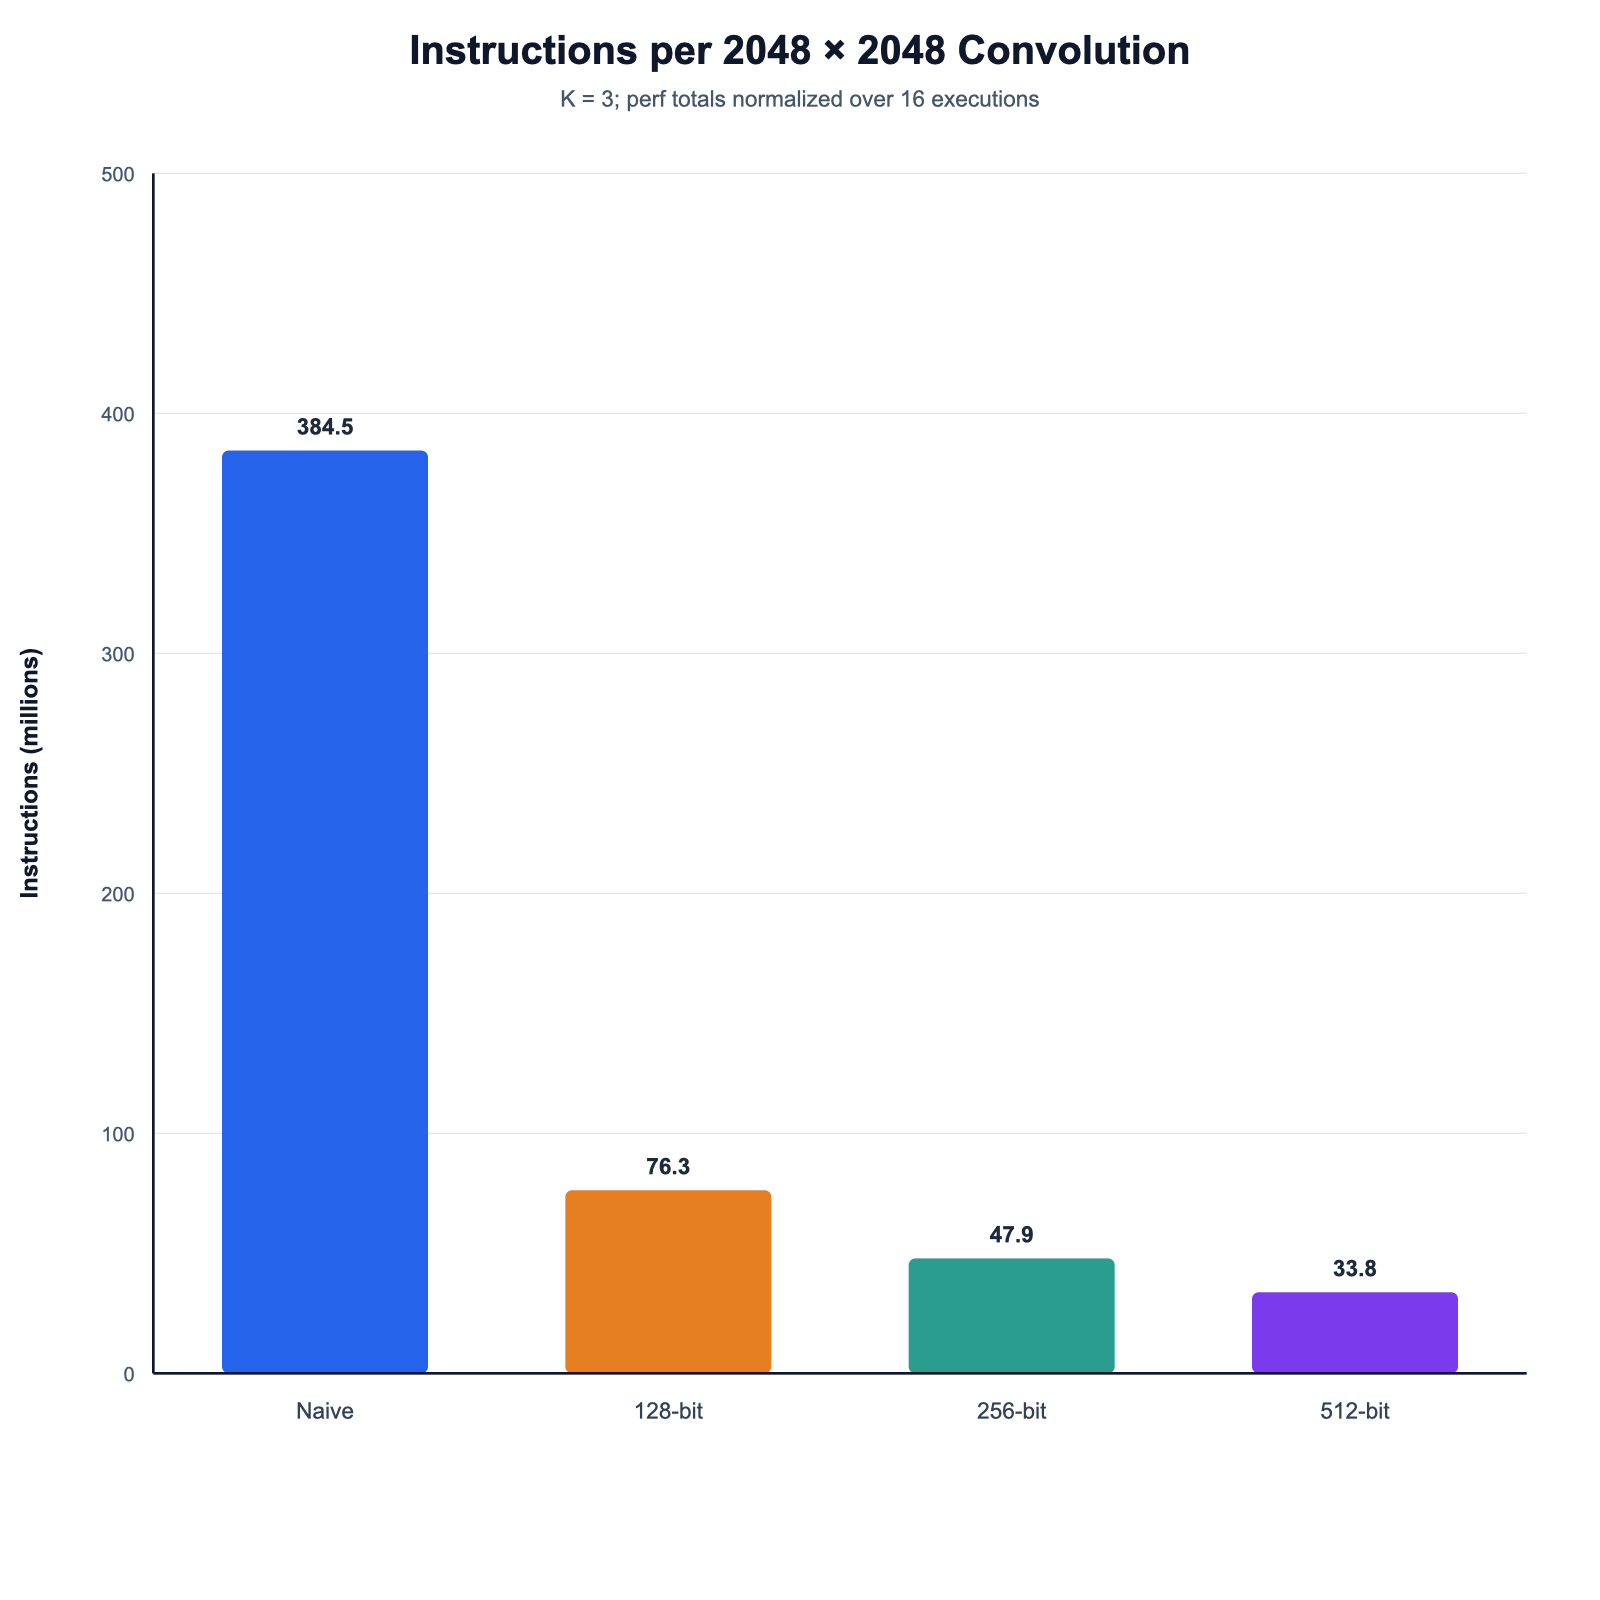
\includegraphics[width=0.56\textwidth]{../plots/task1_simd_instructions.png}
  \caption{Retired instruction count for naive and SIMD-only versions.}
\end{figure}

\subsection{SIMD width and matrix size}

Figure~\ref{fig:simdwidth} uses full-height passes to isolate SIMD from tiling. Wider registers reduce instructions strongly, but runtime speedup approaches $2\times$ for large matrices. At $N=2048$, AVX2 retires about eight times fewer instructions than naive but reaches only 1.97$\times$ speedup. The output is repeatedly read and written for each kernel position, making memory bandwidth and cache capacity the limiting factors.

AVX-512 is fastest for small matrices, but its advantage over AVX2 is negligible at $N=4096$. Wider vectors cannot remove the memory bottleneck and may also reduce sustained core frequency on some processors. AVX2 is therefore the appropriate portable target for the submitted implementation.

\begin{figure}[H]
  \centering
  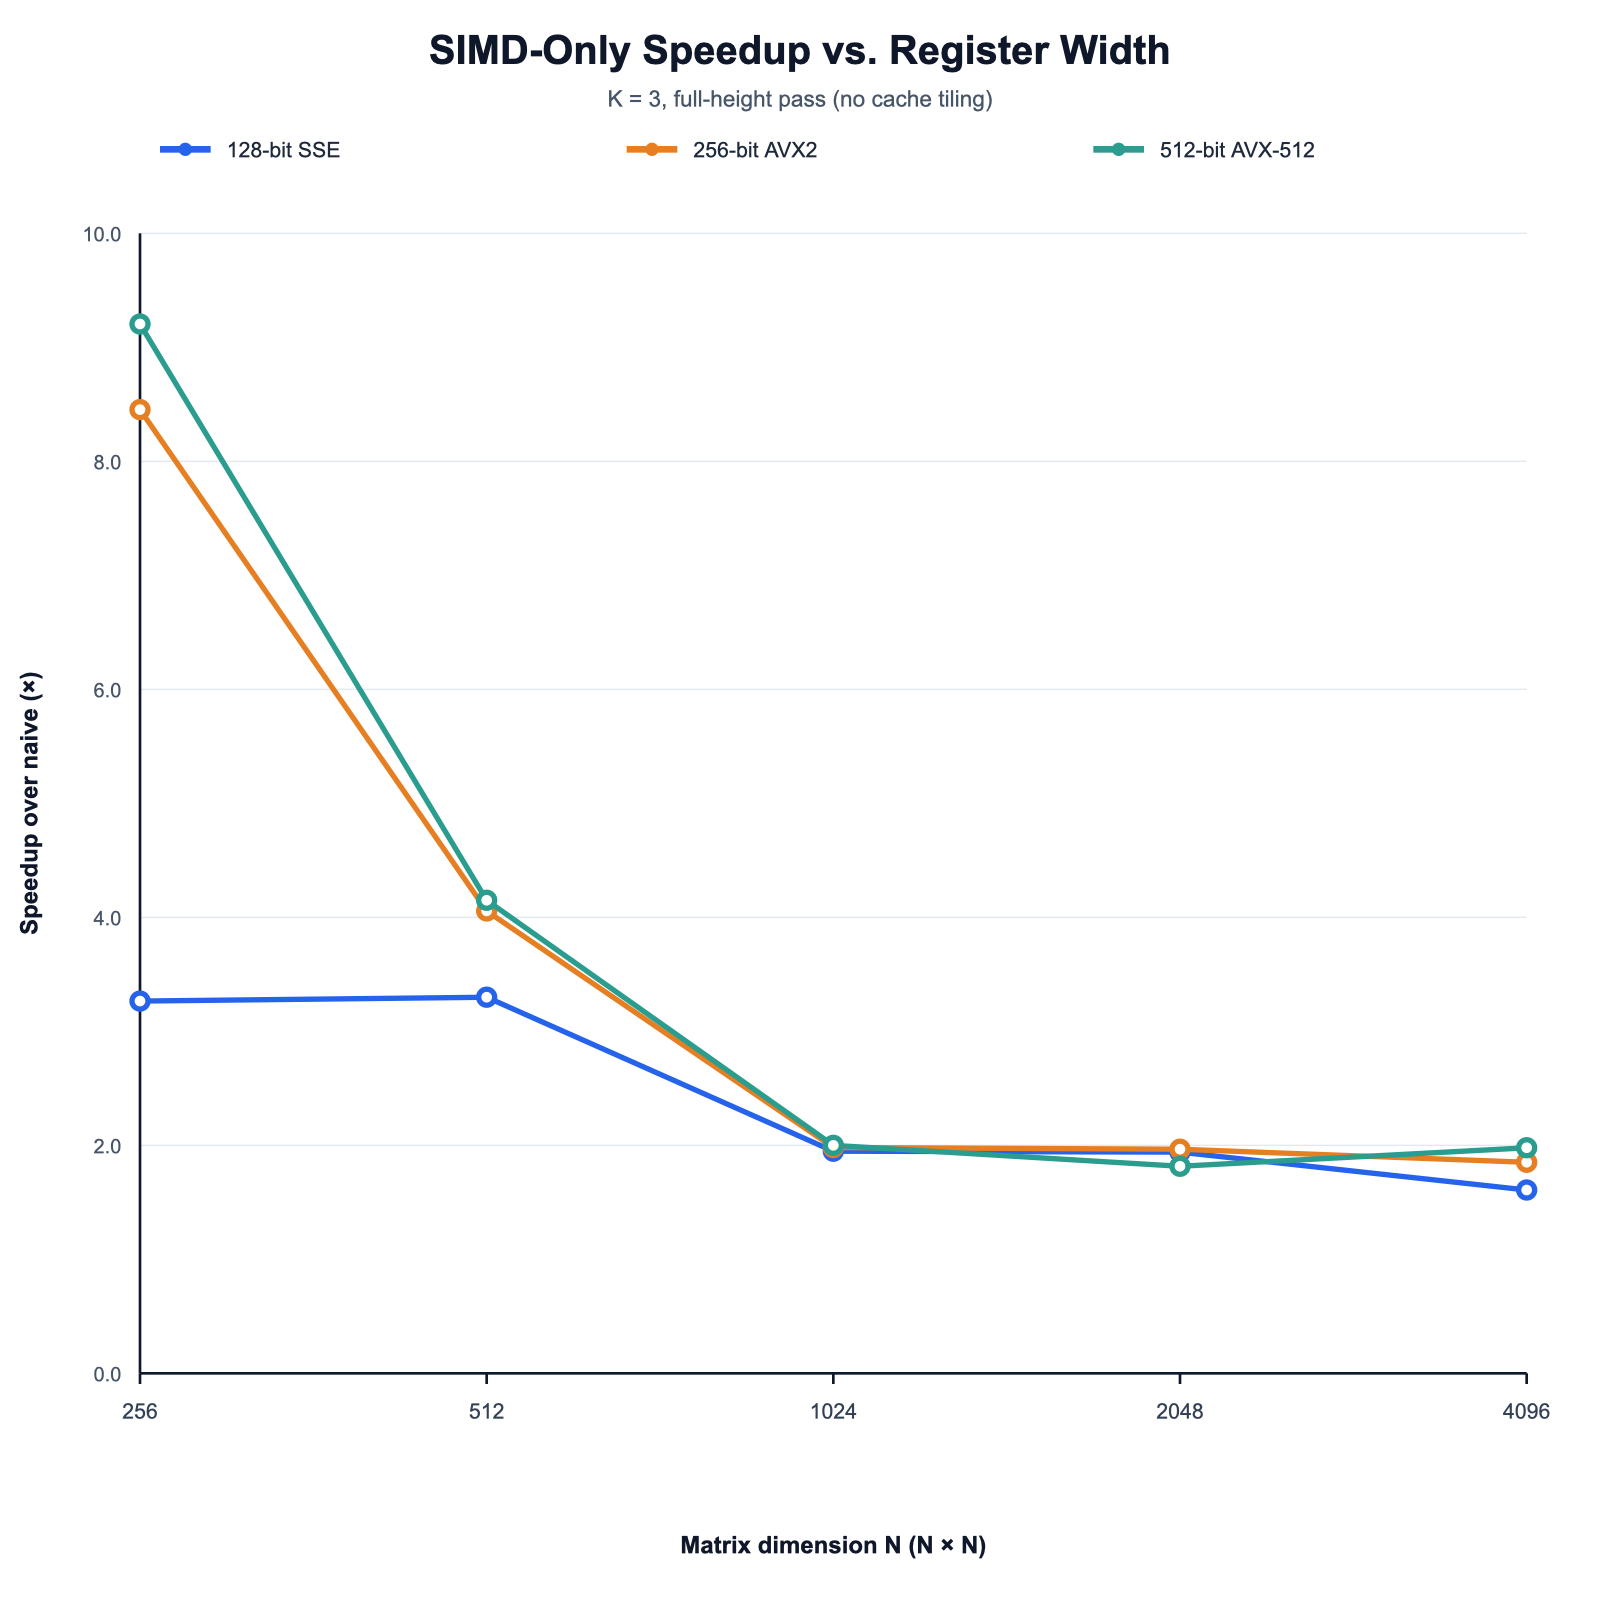
\includegraphics[width=0.83\textwidth]{../plots/task1_simd_width_vs_size.png}
  \caption{SIMD-only speedup for 128-, 256-, and 512-bit registers.}
  \label{fig:simdwidth}
\end{figure}

\clearpage
\section{Task 1D: combined optimization}

The submitted AVX2 stage combines a two-row cache strip with eight-float vector operations. At $N=2048$, pure AVX2 without tiling reaches 1.97$\times$ and scalar tiling reaches 2.63$\times$, whereas tiling plus AVX2 reaches 9.54$\times$. Tiling removes the memory bottleneck that otherwise prevents SIMD throughput from being used effectively.

The final optimized kernel computes four AVX2 vectors, or 32 output columns, together. Four independent accumulators stay in registers while all kernel taps are processed, and each output vector is stored once. This removes the repeated partial-output traffic of the reordered stages and exposes more instruction-level parallelism. The result is 19.95$\times$ at $N=2048$, $K=3$.

Combined speedup decreases at $N=4096$ because the input and output exceed the shared-cache-friendly regime and the virtualized host shows more memory and scheduling pressure. Even there, the optimized kernel remains 7.24$\times$ faster than naive, while reorder and unroll alone are slower than naive.

\subsection{Kernel-size trend}

For $K=1$, setup and vector-loop overhead form a large fraction of the work, so the fully optimized version is not the fastest stage. From $K=3$ onward, register accumulation amortizes the setup and reaches roughly 18--20$\times$. As $K$ grows to 7 and 9, added input traffic and a longer dependency chain slightly reduce speedup, although performance remains well above the scalar stages.

\begin{figure}[H]
  \centering
  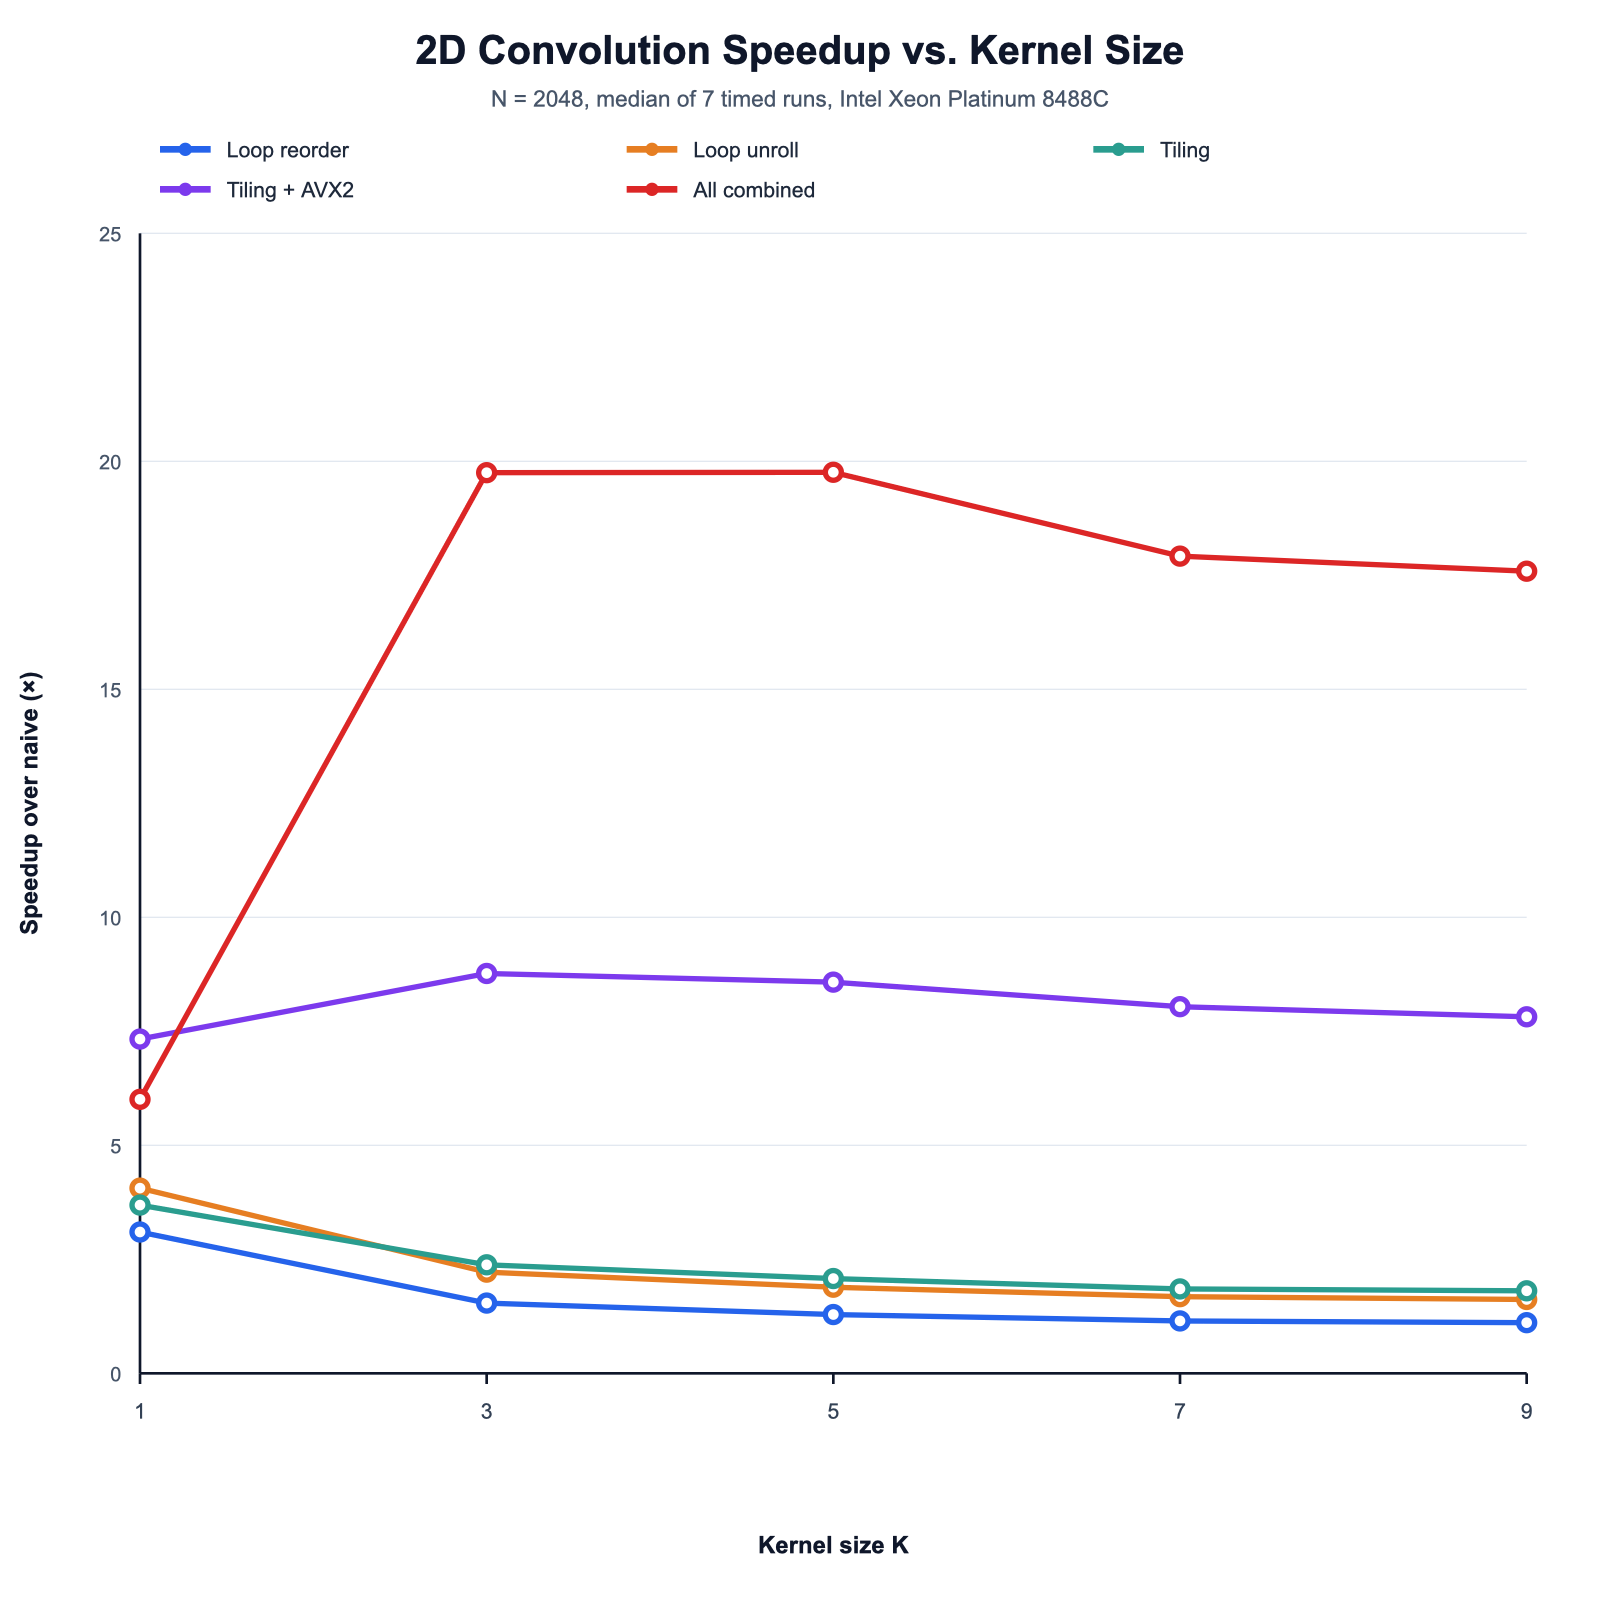
\includegraphics[width=0.66\textwidth]{../plots/task1_speedup_vs_kernel.png}
  \caption{Speedup versus kernel size at a fixed $2048\times2048$ image.}
\end{figure}

\clearpage
\section{Conclusions}

\begin{enumerate}
  \item Loop reordering creates regular unit-stride streams, but repeated full-output passes can become slower than naive once the image outgrows cache.
  \item Eight-way scalar unrolling reduces branch overhead and exposes independent operations, producing a modest gain without reducing memory traffic.
  \item Cache tiling limits reuse distance. A one-row scalar strip best matches the 48 KiB L1-D cache for large tested images; two rows perform best for the AVX2 stage.
  \item SIMD greatly reduces retired instructions, but SIMD alone becomes memory-bound on large images. Instruction reduction therefore does not translate directly into equal runtime speedup.
  \item Tiling and SIMD complement each other. Register-blocked AVX2 accumulation removes repeated output traffic and produces the best result: approximately 20$\times$ on the graded $2048\times2048$, $K=3$ workload.
\end{enumerate}

The final code modifies only the five permitted convolution source files and preserves the supplied build system and compiler flags.

\end{document}
